\documentclass[10pt,a4paper,notitlepage]{article}
\author{Nerea Gonzalez Cordero}
\usepackage[utf8]{inputenc}
\usepackage{amsmath}
\usepackage{amsfonts}
\usepackage{amssymb}
\usepackage[left=3cm,right=2cm,top=2cm]{geometry}
\usepackage{graphicx}

\renewcommand{\baselinestretch}{0.7} %para cambiar el interlineado
%\linespread{0.7} % para cambiar interlineado
\pagestyle{empty} % para quitar números de las páginas

\usepackage{wrapfig}
\usepackage{boxedminipage}

\begin{document}

%{\begin{wrapfigure}{r}{0.25\textwidth}
%	\vspace*{-1cm}
%	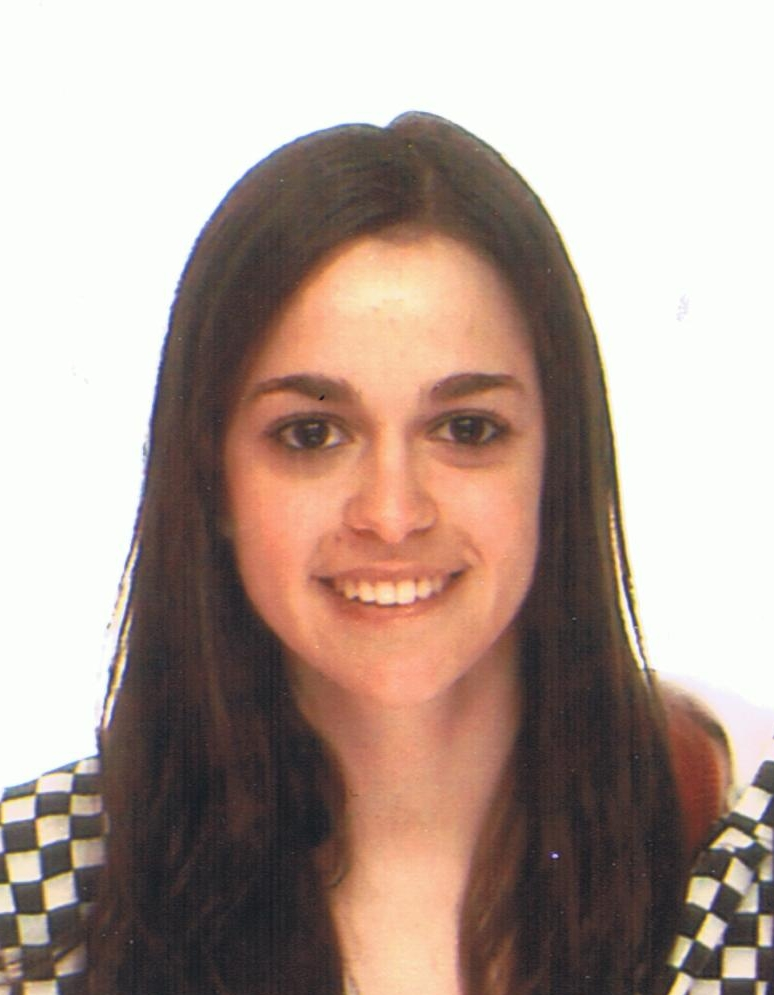
\includegraphics[width=0.20\textwidth]{fotocarnet.jpg}
%\end{wrapfigure}
%\section*{CURRICULUM VITAE}
%\vspace{0.5cm}
%\section*{Nerea González Cordero}
%}
%\vspace{0.5cm}

\noindent
\begin{minipage}[t]{0.75\textwidth}
	\vspace{0pt}
	\section*{CURRICULUM VITAE}
	%\vspace{0.5cm}
	%\section*{Nerea González Cordero}
\end{minipage}
\begin{minipage}[t]{0.25\textwidth}
	\vspace{-20pt}
	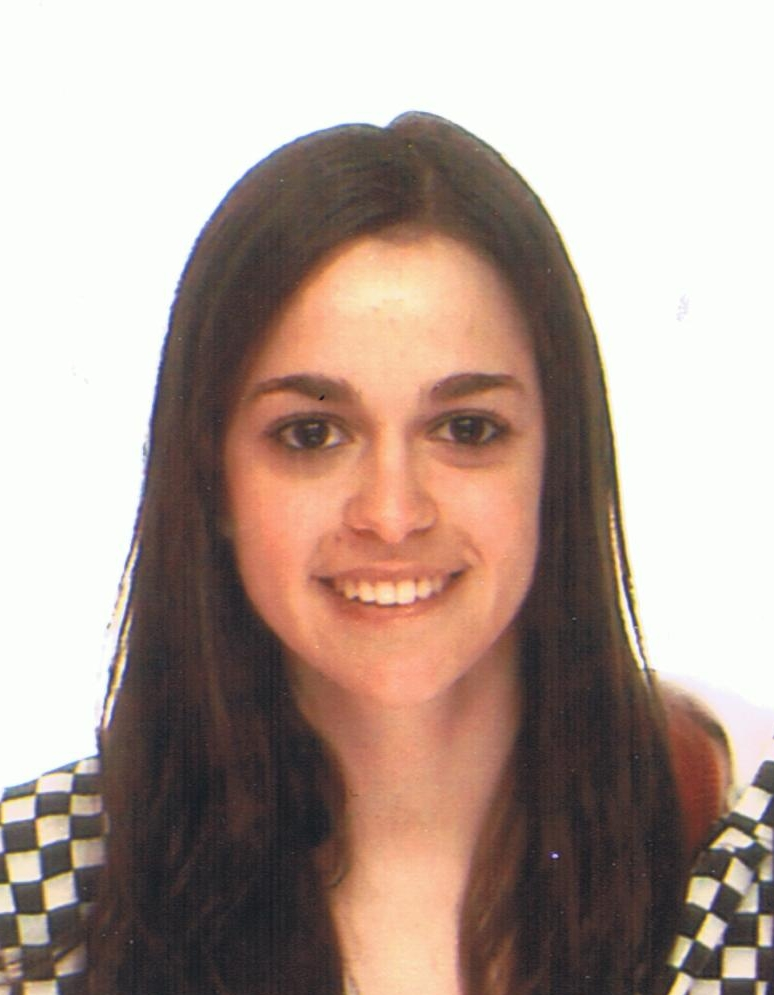
\includegraphics[width=0.64\textwidth]{fotocarnet.jpg}
\end{minipage}

\subsection*{Información Personal:}
\begin{description}
  \item[Nombre:] González Cordero, Nerea
  \item[Dirección:] Calle Los Fueros, 7 - 2ºC, Algorta-Getxo, Vizcaya
  \item[Teléfono:] 696545947
  \item[Correo electrónico:] nerea.gc.92@gmail.com
  \item[Nacionalidad:] Española
  \item[Fecha de nacimiento:] 21/04/1992
\end{description}

\subsection*{Formación Reglada:}
\begin{description}
  \item[2010-2014] Grado en Enfermería en la Escuela Universitaria de Enfermería de Leioa (UPV-EHU).
\end{description}
\begin{description}
  \item[1998-2010] Educación Primaria, Secundaria y Bachillerato en el Colegio Padre Andrés de Urdaneta.
\end{description}

\subsubsection*{Prácticas de Enfermería:}
\begin{itemize}
  \item Residencia municipal de Getxo para personas mayores ``Sagrado Corazón de Jesús''.(2014)
  \item Planta de Medicina Interna, Hospital Universitario de Cruces.(2013)
  \item Centro de Salud de Alango.(2013 y 2014)
  \item Urgencias de ginecología y partos, Hospital Universitario de Cruces.(2013)
  \item Unidad Neonatal, cuidados medios y cuidados intensivos, Hospital Universitario de Cruces.(2013)
  \item Unidad de Enfermedades Infecciosas, Hospital Universitario de Basurto.(2012)
  \item Planta de Enfermedades Respiratorias, Hospital Universitario de Basurto.(2012)
  \item Cardiología, Hospital Universitario de Basurto.(2012)
  \item Unidad de Corta Estancia, Hospital Universitario de Basurto.(2011)
  \item Planta de Urología, Hospital Universitario de Basurto.(2011) 
\end{itemize}

\subsection*{Formación Complementaria:}
\begin{itemize}
  \item 2014: Curso GNU/linux básico I en el centro cívico municipal de San Ignacio.
  \item 2013: Curso de Extinción de Incendios en la Cruz Roja de Bilbao.
  \item 2012-2013: Curso de Auxiliar Técnico de Ambulancia (ATA) en la Cruz Roja con base en Leioa.
  \item 2012: Curso de Primeros Auxilios y DEA en la Cruz Roja de Getxo.
\end{itemize}

\subsubsection*{Idiomas:}
\begin{description}
  \item [Castellano] Lengua materna.
  \item [Inglés] Cursando C1 en la Escuela Oficial de Idiomas de Getxo (2014). Diversas estancias en países de habla inglesa (2006 y 2007 Irlanda, 2008 Malta).
  \item [Euskera] Cursando B1.2 en la Escuela Oficial de Idiomas de Getxo.
  \item [Francés] Conocimiento básico (5 cursos en Educación Secundaria Obligatoria y Bachillerato).
\end{description}

\subsection*{Otros:}
\begin{itemize}
\item Permiso de conducción tipo B. (2011)
\item Conocimiento básico de las Tecnologías de la Información y la Comunicación.
%\item Nadadora en el equipo de natación del Colegio Padre Andrés de Urdaneta. (2001-2007)
\end{itemize}
\end{document}